\chapter*{Introduction}         % ne pas numéroter
\label{chap-introduction}       % étiquette pour renvois
\phantomsection\addcontentsline{toc}{chapter}{\nameref{chap-introduction}} % inclure dans TdM

% Note: This is an un-numbered chapter.

Outline notes:

\begin{outline}
	\1 Challenges of effective control and optimization of comminution (grinding) operations.
	\1 Among these, disturbances, in particular changes in ore properties — difficult to measure accurately in real time, impacts on the downstream process and control systems can be severe \citep{herbst_optimal_1988}.
	\1 Cause-effect chain: Variable ore → variable operation → variable grind → variable recovery → lower recovery \citep{powell_applying_2009}.
	\1 Sources of variability in mining operations: geological characteristics of ore bodies, mining processes such as blasting, material handling, shovelling and trucking. Segregation effects.
	\1 Effects of ore properties on grinding performance (need references).
	\2 Increased hardness/competency → lower breakage rates → increasing hold-up, circulating load → reduced throughput and/or less grinding (TODO: the simulation model apparently contradicts this).
	\2 Particle size distribution → breakage rates in SAG mills → hold up, circulating load → throughput/grind
	\2 Effects on grinding and downstream separation processes (e.g. flotation)
	\2 Grade / grain size → liberation → recovery.
	\2 Density → changes in mill weight/volume estimates (this may be less significant than the first three)
	\1 Figure: Cause-effect diagram.
	\1 Reference and/or include results from Copper Mountain case study (Sijia Liu, 2012).
	\1 SAG mill constraints - grate, throughput, residence time, power, etc. Interplay with secondary grinding.
	\1 Motivations
	\2 realistic disturbance models for simulation
	\2 improve disturbance models for state estimation
	%better characterization of these disturbances in real operations → better models → more realistic simulations → better observers → better control and real-time optimization systems/strategies.
	%\1 Many potential benefits: Improve process control performance (reduced variability, disturbance rejection, adaptive control, robustness (i.e. maintain operating conditions within stable region—esp. w.r.t. SAG mill), → improved process performance (throughput, liberation, power consumption, etc.).
	%\1 Use in upstream in the mining operation to help determine the source of variation and identify process improvements.
\end{outline}

\begin{figure}[htp] \label{fig:cause-effect}
	\centering
	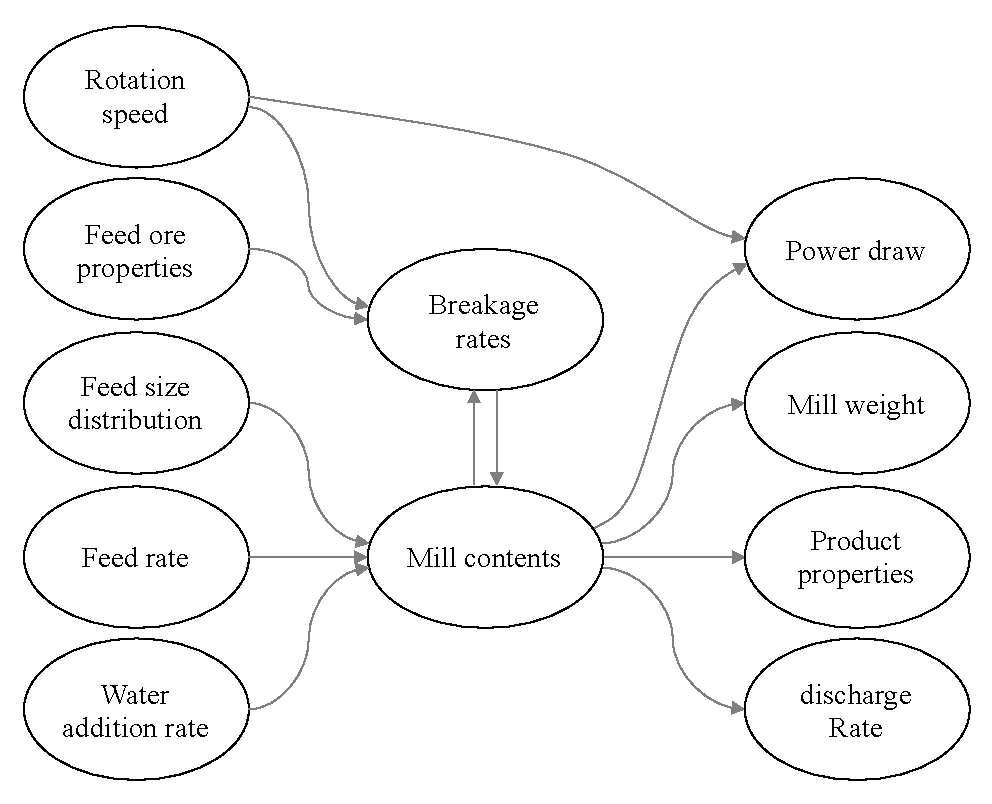
\includegraphics[width=9cm]{images/cause-effect.pdf}
	\caption{Cause and effect diagram}
\end{figure}

Possible references for above:
\begin{outline}
	\1 Herbst et al (1984) - optimal control potential in grinding
	\1 Wei and Craig (2009) - control methods survey, DYNAFRAG simulations.
	\1 Olivier and Craig (2017) - degree of automation survey
	\1 Powell, Mainza (2009) - grind curves
	\1 Hodouin, et al. (2011). Methods for automatic control, observation, and optimization in mineral processing plants.
	\1 Pomerleau et al. (2000) - survey of control
	\1 References on effects of ore properties on grinding performance ?
	\2 Hahne, Palsson, Samskog (2002) - AG effects.
	\1 McClure and Gopaluni (2015) - Overload Detection in Semi-Autogenous Grinding.
	\1 Papers on observers for mineral processing applications — E.g. 
	\2 Olivier, Huang and Craig (2012) - Dual particle filters for state and parameter estimation.
	\2 LeRoux et al (2016) - State and parameter identifiability, EKF observer.
	\2 LeRoux et al (2016) - Nonlinear observability of grinding mill.
	\2 LeRoux et al (2017) - An EKF observer to estimate semi-autogenous grinding mill hold-ups.
	\1 Papers on process control and any including simulations with ore feed disturbances.
	\2 Najim, Hodouin, Desbiens, (1995) simulated an adaptive controller applied to a grinding circuit with a disturbance in the ore hardness (-20\% reduction in breakage rates) and it's effect on the CVs, product P80 and circulating load.
	\2 Chen, Yang, and Li, (2009). Disturbance Observer Based Multi-Variable Control of Ball Mill Grinding Circuits. (They simulated the effects of a 10\% increase in ore hardness on P80 and circulating load).
	\2 Aguila-Camacho, Le Roux, Duarte-Mermoud, Orchard, simulated a fractional order controller with a grinding circuit with a change in the mill feed size distribution.
	\2 Botha, le Roux, Craig, (2018) - Hybrid Non-Linear MPC of a Run-of-Mine Ore Grinding Mill Circuit.
	\2 LeRoux et al (2016) - Non-linear MPC.
\end{outline}

\section*{Disturbances}

Outline notes:

\begin{itemize}
	\item Definition of a disturbance —unmanipulatable inputs to process.
	\item Measured v. unmeasured (and unpredictable)— measured disturbances can be incorporated in a feed-forward control.  Unmeasured disturbances must be estimated in order to reject them.
	\item Importance of considering disturbances in control system design.
	\item Disturbance models and process observers.
	\item \textbf{Some of this section should maybe go in Method chapter}
	\item Two categories of disturbances: Infrequent, always-present.
	\item Infrequent disturbances could have significant impact on process and control systems (MacGregor et al).
	\item Standard approaches to system identification do not consider infrequent disturbances (focus on second order properties)
	\item Need for broader range of disturbance model types and ways to incorporate them in control strategies.
\end{itemize}

\section*{Background and objectives}

This project is part of a three-year research and development project by the \textit{Laboratoire d’observation et d’optimisation des procédés} (LOOP) of the University of Laval, with financial support from the Government of Quebec and Nemaska Lithium Corporation. The overall goal of the project is to determine the extent to which technological innovations could transform the current paradigm of mineral processing which is energy intensive and results in significant greenhouse gas emissions. The project consists of two main initiatives:

\begin{enumerate}
	\item Development of dynamic operating models of production units
	\item Development of circuit configurations, process controls, and real time optimization strategies.
\end{enumerate}

Aligned with the second initiative, the specific goals of this research project are to identify or develop disturbance models and observers tailored specifically to the types of disturbances and measurement challenges that exist in real mineral processing operations.

The specific objectives of this research project are:

\begin{enumerate}
	\item Propose a model for representing disturbances in mineral processing operations
	\item Propose an observer framework using this model.
\end{enumerate}

\section*{Literature review}

Outline notes :

\begin{itemize}
	\item MacGregor et al (1985)
	\item Reference standard approaches to disturbance model design for MPC?  E.g. Badgewell and Muske, Pannochia.
	\item Andersson (1985)
	\item Gustaffson (1993)
	\item Robertson et al (1995, 1998)
	\item Eriksson and Isaksson (1996)
	\item Wong and Lee (2006, 2009).
	\item Branch of research on fault/anomaly detection (Willsky) and limitations vs. state estimation of switching systems.
	\item Papers on state estimation... Blom and Bar Shalom, Ackerson and Fu, Busbaum and Haddad, Jaffer and Gupta, Akashi and Kumamoto,
	\item Hybrid systems (e.g. Sworder and Boyd)
	\item Discrete time Markov Jump Linear systems (MJLS) (Costa 2005 book)
	\item Bemporad on identification of switching systems (e.g. mixed-integer programming)
	\item Problems of observability and Identifiability of Jump Linear Systems (Vidal et al. 2002).
	\item Other estimation methods—particle filtering (Arulampalam, 2002 tutorial).
	\item Control of processes subject to intermittent disturbances. MacGregor, Costa book, Wong and Lee (2000), Camacho et al. 2021?
	%\item What about commercial simulation software (e.g. IDEAS)? What disturbances do they simulate?
\end{itemize}

A comprehensive search of the academic literature was carried out to identify previous work relevant to the project. During this process it became apparent that the number of works related to characterising and identifying realistic disturbances was quite small. With a few exceptions, searches for terms such as `disturbance model' or `disturbance characterisation' tended to result in works dealing with the design of standard stochastic disturbance models, for example \cite{muske_badgwell_disturbance_2002}, and \cite{pannocchia_robust_2003}, or were focussed mainly on detection and diagnosis of disturbances rather than their simulation or modelling, \cite{thornhill_advances_2007} for example. There is a rich body of work on the subject of fault detection which falls into the second category. In these works, models of the process are used to identify when an \textit{unmodelled} disturbance occurs and to determine its source. However, a typical fault detection algorithm does not have a model of the actual disturbance, therefore its operation is suspended once the disturbance occurs. In contrast, the goal of this work is to identify a model that can be used for state estimation in the presence of disturbances, without interruption.

Some of the exceptions were works on disturbances in specific application domains such as wind power generation, bump disturbances in vehicle suspension systems, and wave disturbances in ship movement control.  In these, researchers developed disturbance models tailored to these applications. For example, \cite{papaefthymiou_mcmc_2008} used a Markov-chain Monte Carlo (MCMC) method to identify and model important characteristics of the wind to generate `synthetic' wind data for the purposes of running realistic dynamic simulations of renewable energy generation systems.

Nevertheless, a small number of research papers were discovered dealing with `realistic disturbances' (loosely defined) occurring in continuous industrial processes. These are also sometimes broadly referred to as `deterministic disturbances' to distinguish them from standard disturbance models based on zero-mean random noise signals (which are truly random in the sense that they are independent and identically-distributed).

\section*{Randomly-occurring deterministic disturbances} \label{RODDs}

In 1984, \cite{macgregor_duality_1984} introduced the concept of the \textit{randomly-occurring deterministic disturbance} (RODD). This is a family of stochastic processes useful for modelling deterministic disturbances commonly encountered in real industrial processes. Three types of RODD process are described by MacGregor and co-workers. One produces infrequently-occurring step changes, another produces a series of ramps, and a third produces a signal consisting of a series of exponential changes. One example of a real-world disturbances that might be represented by these models is that of an unanticipated set-point change made by an operator. Another is an sudden unexpected change to the load on a system. While these disturbances may be deterministic, the key issue is that they are not predictable or measurable by the control system. Therefore, simulating them with a stochastic process driven by a random variable is a reasonable way to emulate their unpredictability for the purposes of control system design.

The structural form of a RODD model is an \textit{autoregressive integrated moving average} (ARIMA) process fed by a special \textit{random shock} signal which has the value 0 most of the time but occasionally, according to a defined probability, has a value sampled from a normal distribution. Depending on the chosen ARIMA process model, this can be used to simulate the different types of RODD disturbances which may act on a process. The details of the RODD model are described in section \ref{subsec-RODD}.

MacGregor and coworkers also showed that the optimal control law derived for a process perturbed by a RODD is no different than that which would be derived for a process subject to a standard stochastic noise.  This is due to the common ARIMA structure of both models and the fact that the expected value (i.e. mean) of the random shock signal is zero as it is for a Gaussian noise. As a result, it is well-suited for use in process control design. For this reason, and in the absence of other alternatives, the RODD disturbance model became a focus of this research project.

\section*{Detection and estimation of RODD disturbances}\label{detection_RODDs}

Traditional filtering methods such as Kalman filters are unable to efficiently estimate RODD disturbances due to the inevitable trade-off that must be made between the ability to track a disturbance when it occurs and the sensitivity to noise \cite{robertson_detection_1995}.

Prior work in the field of process monitoring focused on the problem of fault detection. The disadvantage of these methods was that, once a fault is detected, the estimation process stops, and some sort of corrective action is required before the filters can be restarted. 

In their 1995 paper, Robertson, Kesavan and Lee \cite{robertson_detection_1995} described how unmeasured RODD disturbances perturbing a system can be estimated online using a \textit{multi-model} observer approach that is effective over an extended period of time during which any combination of several disturbances may occur.

Multi-model filtering approaches involve simultaneously computing multiple independent filters with different parameters and then combining the estimates from these filters to produce a better estimate of the system states \cite{jaffer_estimation_1971, buxbaum_recursive_1970, tugnait_detection_1982}.

Unlike the random shock signal defined by MacGregor and co., Robertson and co. use a signal that is sampled from one of two normal distributions, one with a low variance and the other with a much higher variance. This means that the probability density of the shock signal is conditionally Gaussian, whereas the shock signal used by MacGregor and co. has a non-smooth (i.e. degenerate) probability density function.

Since the sequence of past random shocks is not known, each filter's state estimate is calculated assuming a different sequence of past possible shocks. The estimates of some filters are therefore better than those of others, depending on how closely the shock indicator sequences match the disturbances that actually occurred. The overall best estimate of the states is computed by calculating the conditional probabilities of each indicator sequence given the available measurement data, and this estimate is updated recursively each sample period using Bayesian inference.

Due to practical limitations, the optimal multi-model approach cannot be implemented and some kind of approximation is needed to limit the number of filters required. Practical multi-model observers are therefore referred to as \textit{sub-optimal}. Robertson and coworkers propose using a combination of three specific approximations when estimating RODD disturbances.

The first is based on the assumption that correctly estimating the exact timing of RODD disturbances is not important and therefore a filter that assumes a shock occurred within a short period close to the actual occurrence will be adequate. This is based on the observation that when the correction gain of a Kalman filter is increased at time $k$ due to the assumption of a shock occurrence, it tends to remain large for several sample periods thereafter.

The second approximation is based on the assumption that RODD disturbances occur infrequently and it is quite unlikely that two or more shocks occur within a short time period. This further reduces the number of filters required, especially in systems subject to multiple independent disturbances.

The third approximation is referred to as \textit{filter fusion} or the \textit{generalized pseudo-Bayes algorithm} \cite{jaffer_estimation_1971, buxbaum_recursive_1970, tugnait_detection_1982}. This is based on the assumption that only differences in the recent values of the shock indicator sequence affect the state estimates. Therefore, sequences whose last $f$ terms are the same can be combined. In other words, the length of the unique sequences which must be maintained is limited to the previous $f$ sample periods.

Robertson and coworkers present results of simulating their sub-optimal multi-model observer on a 2-input, 2-output, non-linear dynamical system representing a continuous stirred-tank reactor (CSTR) process. They show the estimates produced by the multi-model approach compared with two single extended Kalman filters (EKF) with different noise parameters. The first of the single EKFs is sensitive to the measurement noise and the second is slow to respond to the RODD step disturbances, while the multiple-model observer appears to perform better than either single EKF in the example simulations.

A year later, Eriksson and Isaksson \cite{eriksson_classification_1996} present results of using an adaptive multi-model approach to estimate \textit{infrequently-occurring disturbances}. They utilize the \textit{adaptive forgetting through multiple models} (AFMM) algorithm by Andersson \cite{andersson_adaptive_1985} and also previously described by Gustafsson \cite{gustafsson_estimation_1993}. The AFMM algorithm employs a technique called \textit{sequence pruning} \cite{tugnait_detection_1982}, in contrast to the sequence merging or fusion technique used by Robertson and co.\cite{blom_interacting_1988}.

Sequence pruning is the online deletion of sequences that have a low probability given the current measurements. The deleted sequences are replaced by new sequences to represent the possible branches of the most likely sequence at the next sample time. For example, for a system with one infrequently occurring input disturbance, the most likely shock sequence at the next sample time is the shock sequence estimated to be most likely at the current time extended by the addition of a zero to indicate no shock at the next sample time. However, a shock could occur in the next time period. To account for this possibility, a new shock sequence is generated by making a copy of the current most likely sequence and its associated filter and extending it assuming a shock at the next sample time. This new sequence and filter replace the least likely sequence and observer. Thus, the total number of sequences and independent filters that need to be maintained remains constant. Note that in the case of systems with more than one input disturbance, the number of possible branches of the most likely sequence is higher, and therefore a larger number of sequences and filters will be replaced each time step.

There is one restriction to this pruning rule. A sequence created at sample time $k$ cannot be deleted until sample time $k+n_{min}$ where $n_{min}$ is a \textit{minimum life length} parameter. This is necessary because it can take several sample periods before the filter estimates respond to the change and thus the conditional probability of the new sequence is established.

The AFMM algorithm also includes a procedure for online estimation of the measurement noise covariance, using a forgetting factor to control the speed of adaptation of the estimate.\cite{andersson_adaptive_1985}

In Robertson and co., the RODD disturbance model is assumed to be known. This is also the case in Eriksson and Isaksson's paper, however, Eriksson and Isaksson show how the estimation procedure can be extended to discriminate between two possible disturbance hypotheses. They consider the example of determining whether a step disturbance is affecting the output or the input of the process, assuming it is actually present at either but not both simultaneously.

Two sets of Kalman filters are run simultaneously, one set with the infrequently-occurring disturbances modelled at the input of the process and the other set with them modelled at the output. The conditional probabilities of all filter models are calculated every sample time and normalized across both sets of filters.  Thus an online estimate can be made of which disturbance hypothesis is most likely (i.e. an input or output disturbance) as well as an estimate of the magnitude of the disturbance. They provide results from simulated examples and a laboratory experiment to show that the AFMM method correctly estimates the disturbance actually present in each case.

Robertson and Lee published a second paper in 1998. In this paper they list Anderson \cite{andersson_adaptive_1985} among the references on multiple-model algorithms.  However, the approach and sub-optimal method used is essentially the same as in their 1995 paper, with only slightly different terminology used (`infrequently occurring abrupt disturbances' instead of `randomly occurring deterministic disturbances'). 

However, a different non-linear system (a 3-state model of a heptane to toluene aromatization process) is used for the numerical example and, importantly, this time sum-of-squared errors for the parameter estimates are presented averaged over 50 Monte Carlo simulations, so it is easier to compare the different methods. They compare their sub-optimal method with a single EKF and with the generalized pseudo-Bayes (GPB) algorithm (without sub-optimal modifications).

The results show that their sub-optimal filter does 35 percent better than either the EKF or the GPB algorithm. This is simply because their filter has a horizon of 90 minutes (using 22 filters), whereas the standard GPB algorithm has a horizon of only 2 minutes (using 16 filters) so there is not enough time for it to detect changes before the filters are fused.

\section*{Disturbance modeling using hidden Markov models}
\label{hidden_markov_models}

Outline notes:

\begin{itemize}
	\item Wong and Lee proposed a generalized framework for modeling realistic disturbance processes which have both continuous and discrete (i.e. modal) dynamics \citep{wong_disturbance_2007}.
	\item The mode transitions are described by a finite-state \textit{Markov chain}.
	\item The model generating the Markov chain is referred to as a \textit{hidden Markov model} (HMM) because it is unknown and must be inferred from available noisy measurements.
	\item The combined system including discrete and continuous dynamics is termed a \textit{Markov jump linear system} (MJLS) \citep{costa_discrete-time_2005}.
	\item Wong and Lee point out that the application of HMM's and MJLS's in science and engineering is not novel and refer readers to the references in \cite{costa_discrete-time_2005} for prior work by the control community. Nevertheless, they claim that the use of HMMs for disturbance modeling prior to 2007 was limited.
	\item They also note that the RODD disturbance model of Robertson and Lee, and other methods assuming noise inputs described by \textit{mixture-of-Gaussians} (MOG), can be considered special cases of the MJLS.
	\item Unlike Robertson and Lee, who focused on state estimation, Wong and Lee are interested in identification of the model in the presence of non-stationary noise.
	\item Wong and Lee show how the plant and Markov chain parameters may be simultaneously estimated by \textit{maximum likelihood estimation}, specifically, using the expectation maximization (EM) algorithm (see section \ref{mle}).
	\item In their numerical examples, Wong and Lee use a second-order generalized pseudo-Bayesian (GPB2)  method for state estimation \citep{bar-shalom_estimation_1993} (see section \ref{gpba}).
	\item The first example in their 2007 paper, is a disturbance that switches infrequently between a white noise and an integrated white noise.
	\item They compared the prediction errors of a GPB2 observer using the identified MJLS model to those of the best observer with a stationary (i.e. non-switching) model, as well as to those of a GPB2 observer which uses the actual system model.
	\item The 1-step-ahead prediction errors of the GBP2 with the identified model were 26 percent lower than the optimal stationary-model observer and only 7 percent worse than those of the GBP2 with the true model.
	\item These results are averages over 500 simulated realizations, each of 2000 sample periods in length.
	\item The second example is a `soft-sensor' approach for inferential control where the system is subjected to two integrated noise disturbances at the output, each switching between two noise levels with certain probabilities. In this example, the simulation results indicated that the 1-step-ahead prediction errors of the GPB2 observer with the identified model were only 6 percent higher than a GPB2 observer with the true model.
	\item The main limitation of the results presented in the 2007 paper is that they only test the method on systems which switch only in their noise parameters.
	\item The other limitation that they acknowledge, is that the MLE optimization is non-convex and hence may not converge to the global optimum. To mitigate this problem, they chose initial values `suitably close' to the true system parameters.
	\item Although Wong and Lee do not refer to it, it's worth noting that Elliott, Aggoun, and Moore wrote a book on hidden Markov models for estimation and control in 1995 \cite{elliott_hidden_1995}. A central theme of this book is use of so-called \textit{reference probability methods} for optimal estimation and control which they claim are accessible to non-specialists.
	\item Reference probability methods involve a change of probability measure (they are also known as the \textit{measure change approach}) which allows the original estimation and control problem to be reformulated so that well-known results for \textit{identically and independently distributed} (i.i.d.) random variables can be applied, thus simplifying the analysis and the computational complexity. \emph{TODO}: where does this approach fit in with the other concepts (e.g. in Costa's book) and is it still relevant today?
\end{itemize}

\section*{The hidden Markov model for process control}
\label{hmm_control}

Outline notes:

\begin{itemize}
	\item Wong and Lee's 2009 paper \cite{wong_realistic_2009} goes further than their 2007 paper \cite{wong_disturbance_2007} by demonstrating how the proposed HMM-based disturbance framework can be integrated into existing model-based control formulations.
	\item After introducing the HMM framework again, they present 3 numerical examples demonstrating the use of the framework in process control methods and applications, including one to mitigate the impact of highly-varying feed streams entering an ethanol-producing bioreactor.
	\item They provide only a brief review of system identification methods for Markov jump systems and note that it was still an open area of research at the time.
	\item Due to the difficulties of MJLS identification, they bypass the issue in this paper, and assume that the system, noise and Markov parameters are available.
	\item As in the 2007 paper, they use the second order Generalized Pseudo-Bayesian algorithm (GPB2) developed by Bar-Shalom \cite{bar-shalom_estimation_1993}.
	\item Although they don't use it, Wong and Lee also mention the interacting multiple model (IMM) algorithm which they say has a similar performance as GPB2 but at the computational cost of GBP1 \cite{wong_realistic_2009}. \textbf{TODO}: Need to see where this fits in.
	\item The GPB2 algorithm is a recursive estimation scheme, characterized by `branching' and `merging' steps. Wong and Lee provide a simple numerical example of the algorithm including plots of the output and state estimates. Refer to Fig. 3 in \cite{wong_realistic_2009}.
	\item The first of the three examples in the 2009 paper demonstrates the use of the HMM disturbance framework for offset-free linear model predictive control (LMPC) on a single-input, single-output system.
	\item Four simulation scenarios are considered for this example: low input noise compared to output noise, high input noise compared to output noise, similar input and output noise levels, and switching levels of input and output noise (all simulations were run with negligible measurement noise).
	\item In order to investigate model-plant mismtch, four different model-predictive controller/estimator pairs were constructed: one with an output disturbance only, one with only an input disturbance, one with both input and output disturbances, and the fourth with switching behaviour (using the GPB2 estimator).
	\item For each of the four simulation scenarios, 500 realizations, each of duration 500 sample periods, were run and a controller coupled with a time-varying Kalman filter assuming perfect knowledge of the true simulation regime was simulated for benchmarking purposes.
	\item Each controller is evaluated by the average ratio of its squared-tracking error and that of the benchmarking controller/estimator.
	\item The simulation results show that the proposed MPC designed with the HMM model and GPB2 estimator yields the best performance over all simulation scenarios.
	\item Example 2 demonstrates the closed-loop performance of the HMM control approach in detecting and rejecting deterministic step changes.
	\item The controller's performance is compared to a well-tuned controller based on the \textit{integrated white noise} (IWN) approach to rejecting such perturbations.
	\item The results show that the HMM framework achieves an increase of only 6 percent in the error when compared to the ideal full-feedback controller, and yields better performance than a well-tuned IWN-based estimator.
	\item The third example concerns the control of a nonlinear ethanol fermentation process simulation model where the HMM framework is used to represent the highly-varying nature of the feed concentrations.
	\item The glucose concentrations entering the process are modelled as fluctuating among several mean levels (low, mid and high) and the transitions are governed by a Markov chain.  The problem is such that the regime transitions are infrequent since changes in feed type/quality tend to occur on time scales that are longer than that of the plant’s dynamics.
	\item A \textit{sequentially-linearized MPC}, which is a computationally attractive alternative to a full non-linear MPC implementation \cite{lee_extended_1994}, is used to evaluate the closed-loop performance.
	\item The effect of different types of feedback is compared: Full state feedback including the Markov decision variable; Markov decision variable and output feedback only, and output feedback only (corrupted by measurement noise).
	\item As in the previous example, a controller/estimator pair that operates on the common assumption that the disturbance is integrated white noise (IWN) is used as a benchmark.
	\item Not surprisingly, the results indicate that the amount of information available to the controller determines the closed-loop performance, especially, knowledge of the Markov state trajectory. However, all three HMM-based approaches are better than the benchmark closed-loop system relying on the output measurements only.
	\item The authors concluded that the benefits of an HMM-based disturbance framework are ``most immediately reaped" by incorporating them within existing control methodologies such as MPC, as opposed to the optimal control policies developed specifically for Markov jump systems, such as those described in \cite{costa_discrete-time_2005}.
	\item Finally, they stated that the development of systematic model identification methods and more robust control algorithms for Markov jump systems was the focus of their ongoing research.
	\item In 2011, Wong and Lee published a conference paper on the HMM framework for disturbance modelling in which they present the framework again. Again they use the GPB2 algorithm for sub-optimal filtering and present results of two numerical examples. One for state estimation with abruptly changing feed conditions for a `second generation' bioethanol fermentor, and the second for the case of tracking stiction in a mechanical valve, which is a non-trivial detection problem.
	\item As in the previous papers, the results show better performance for the HMM-based approaches.
\end{itemize}


\section*{Contributions of this research}

The main contributions of this research are:

\begin{enumerate}
	\item A review of academic literature pertaining to `realistic' disturbance modelling and state estimation in industrial process operations.
	\item Evaluation of the capabilities of two multi-model observer algorithms by simulations in MATLAB.
	\item Evaluation of the performance of one of the multi-model observers applied to state estimation of a simulated grinding process.
	\item Evaluation of the benefits of one of the multi-model observers as part of a simulated control system applied to the simulated grinding process.
	\item T.b.d.: A case study of the application of model identification techniques to characterise disturbances using data from a real industrial operation.
\end{enumerate}

\section*{Organisation of this report}

Chapter 1 describes the methods used in the research including the disturbance model, the observer designs and the grinding simulation model used for evaluation of one observer.  Chapter 2 describes the simulations carried out to demonstrate the disturbance model and to evaluate the performance of the observers (TODO: And to estimate the potential benefits?). Chapter 3 describes simulations carried out to test some of the possible methods to identify and characterise disturbances from measurement data.
